\subsection{Implementation and dependencies}
\bioptim is the top layer of a succession of libraries (\biorbd: dynamics and MSK modeling; \casadi: automatic differentiation; \ipopt/\acados: optimization; \bioviz: visualization).
Within this software suite, \bioptim 's main role is to shape the problem to allow its dependencies to communicate efficiently, while providing an intuitive and flexible interface to the user (Fig.~\ref{fig:dependencies}).
Therefore, it was written in Python for its flexibility and its widespread use among researchers.
However, all intensive calculations behind the interface are performed in C/C++, keeping \bioptim both fast and easy to customize.

\begin{figure}[t!]
\centering
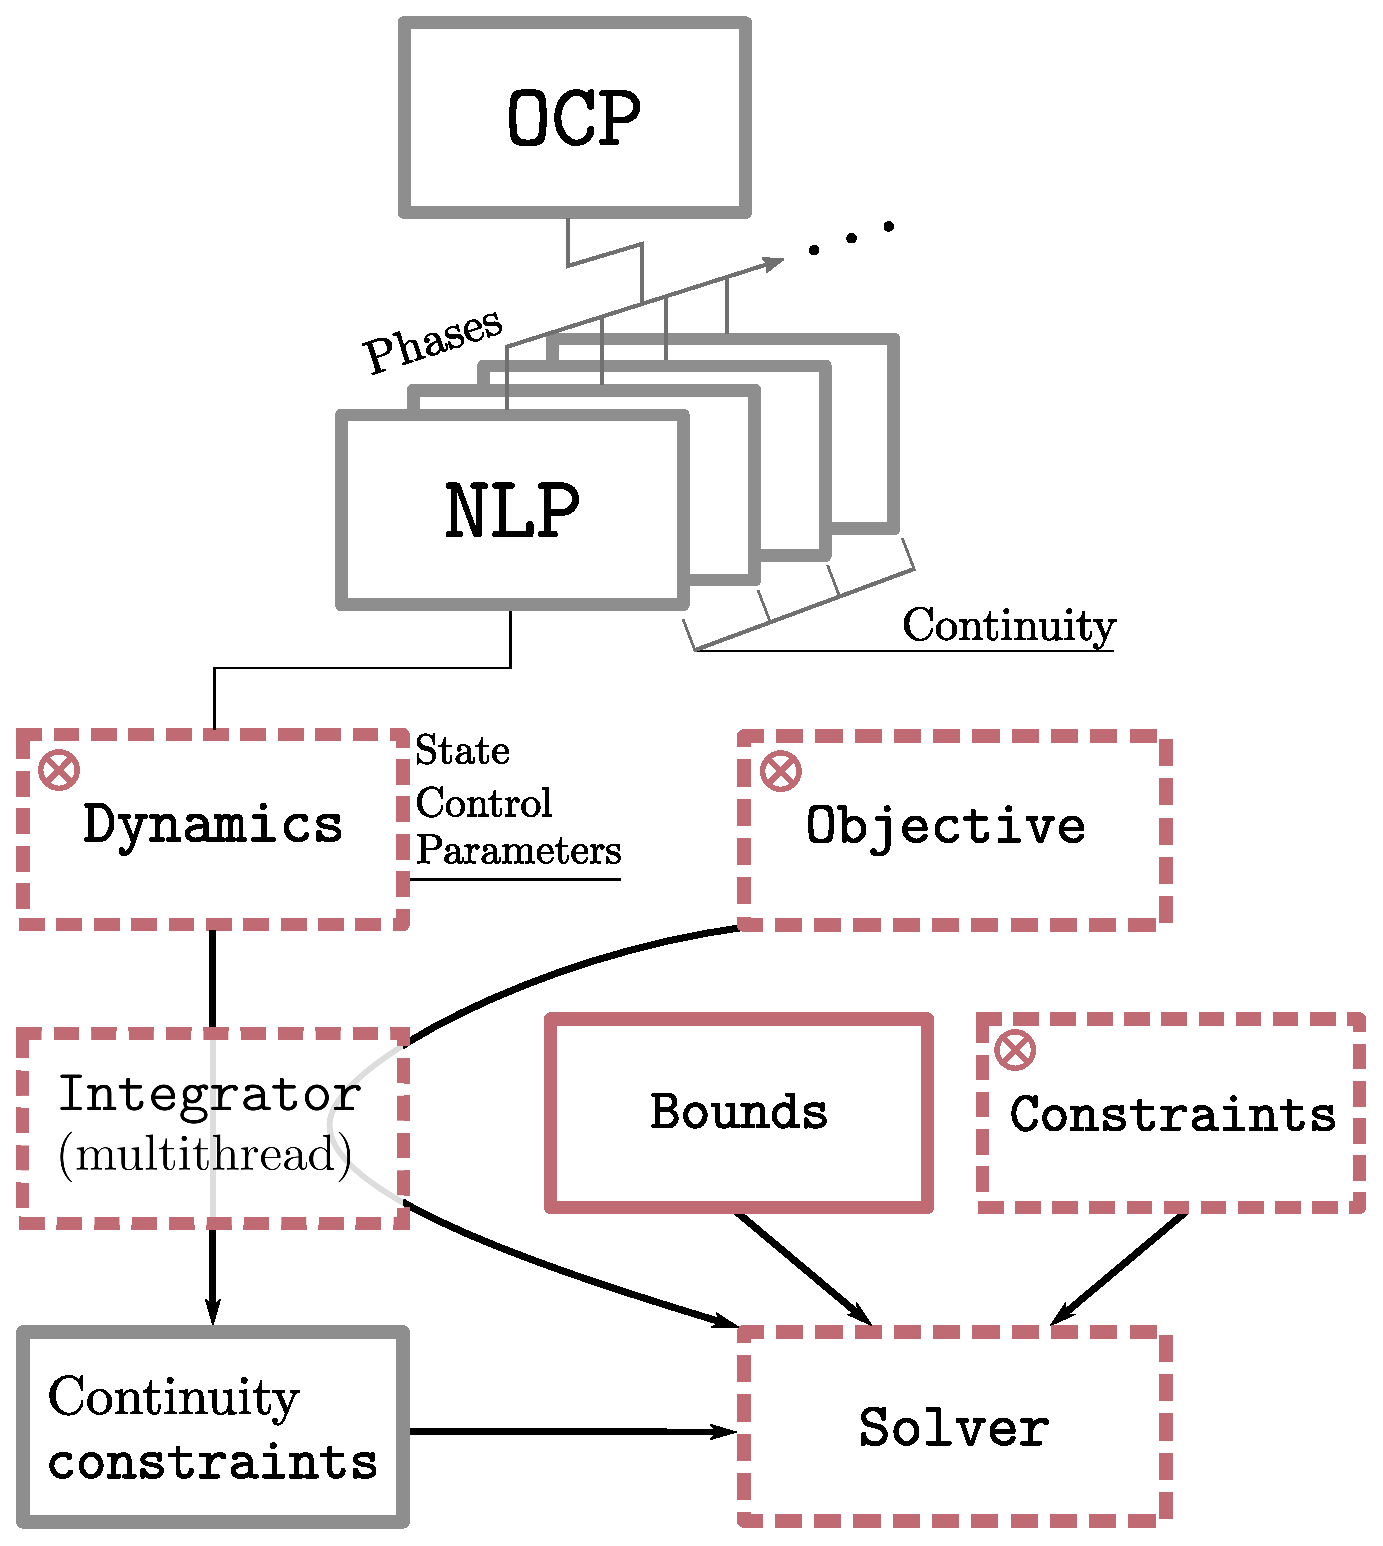
\includegraphics[width=0.9\columnwidth]{figures/design.eps}
\caption{\bioptim design \comment{flowchart}{D'après moi, il manque PhaseTransition dans le bout de NLP, mais je ne suis pas sûr comment le mettre. Je ne pense pas que les flèches avec l'étoile soient vraiment visibles... Peut-être mettre directement l'étoile à coté du mot (Objective*)? Soothing defects refère à la contrainte de continuité, c'est bien ça? Si on met ça (et je pense que ça devrait être un peu plus clair), il faudrait peut-être mettre aussi les boundaries...)}.}
\label{fig:dependencies}
\vspace*{-0.5cm}
\end{figure}


\subsection{Design}
\bioptim shapes and solves optimal control problems whose two required entries are a model (.\textit{bioMod} file) and an OCP.
The model file contains the geometrical characteristics, the segment inertias, the markers, the actuators of the model (muscles and joint torques possibly with torque/angle/velocity relationships) as well as bounds on joint kinematics and torques. 
It also allows the user to design or import meshes for visualization purposes.
The OCP consists in a combination of nonlinear problems (NLPs) that allows for the formulation of multi-staged OCPs. 
Each NLP has the following attributes: a dynamics type, an objective function set, a constraint set, a number of shooting points, a duration of the problem, initial guesses and variables bounds.
Based on these inputs, \bioptim properly sets up the multiple shooting transcription of the OCP, with appropriate continuity constraints (between the shooting nodes and the phases) and shapes it up to feed the chosen nonlinear solver (\ipopt or \acados). 

\subsubsection{Dynamics}
The dynamics defines which variables are states ($\state$), controls ($\control$) and parameters ($\param$), the latter being time-independent.
Then, it implements the ordinary differential equation governing the state dynamics:

\[
\dstate = f(\state, \control, \param).
\addtag
\label{eq:state_transition}
\]

\noindent More than 10 dynamics are implemented in \bioptim \footnote{\href{https://github.com/pyomeca/bioptim/blob/master/bioptim/dynamics/dynamics_functions.py}{github link}}, among which the controls can be muscle excitations, muscle activations and/or joint torques, the states can be muscle activations and/or joint kinematics.
They can include contact points, external forces, etc.
Even if these dynamics types exhaustively span the current usages in biomechanics, a custom dynamics type is also pre-implemented to easily customize problems.

\subsubsection{Objective functions}
In line with the optimal control formalism, there are two main types of objective functions, namely Lagrange and Mayer. 
Lagrange types are running objectives, integrated over the NLP duration. Mayer types are time-specific objectives. 
Classically, they correspond to a terminal objective, but to be more versatile, they can be defined at any instant in \bioptim.

Objective functions can depend on any of the optimization variable, \textit{i.e.} the controls, the states, the parameters and the duration of the problem. 
A lot of objective function types are already implemented in \bioptim ($>\!20$), among which tracking\:/\:minimizing, on states\:/\:controls\:/\:markers\:/\:contact\:forces\:/\:problem\:duration, etc. 
Should one go missing, a custom objective type is also possible to define.

When declaring the desired list of objective functions for a given NLP, each objective function type is associated with a weight, and the user can choose on which components of the vector variables the objective must apply. 
If applicable (for tracking objective functions mainly), the user must also specify the numerical target of the objective.

\subsubsection{Constraints}
Classically, constraints are hard penalties of the optimization problem, i.e., a solution will not be considered optimal, unless every constraint (equality or inequality) is met.
The \texttt{Constraint} class contains a variety of already implemented constraints.
Some of them are specific functions, commonly useful in biomechanical problems (e.g. non-slipping contact point, non-linear bounds on torque depending on the state, etc.), the others  
have their equivalent in the \texttt{ObjectiveFunction} class.
Should one go missing, a custom constraint type is also possible to define.

\subsubsection{Bounds}
Essentially, the \texttt{Bounds} are constraints directly related to the states, the controls and the parameters.
They are useful for defining model-related constraints such as kinematic, torque or muscle excitation\:/\:activation limits. 


\comment{}{Shooting points, phase time, initial guesses?}
